
% this file is called up by thesis.tex
% content in this file will be fed into the main document

%: ----------------------- introduction file header -----------------------

%*************************************************************************
%Quote
\begin{savequote}[50mm]
‘‘El cosmos es todo lo que es, todo lo que fue y todo lo que será. ’’
Nuestras 
más ligeras contemplaciones del cosmos nos hacen estremecer: Sentimos como 
un cosquilleo nos llena los nervios, una voz muda, una ligera sensación como
de un recuerdo lejano o como si cayéramos desde gran altura. Sabemos que nos
aproximamos al más grande de los misterios.’’
\qauthor{Carl Sagan}
\end{savequote}
%*************************************************************************

\chapter{Marco Teórico}
\label{cha:Theoretical Framework}

% the code below specifies where the figures are stored
\ifpdf
    \graphicspath{{2_state_of_the_art/figures/PNG/}{2_state_of_the_art/figures/PDF/}{2_state_of_the_art/figures/}}
\else
    \graphicspath{{2_state_of_the_art/figures/EPS/}{2_state_of_the_art/figures/}}
\fi


%*************************************************************************
Este capítulo se concentra en abarcar de forma autocontenida y resumida 
todo el marco teórico necesario para el estudio del universo a gran escala,
pasando por los modelos simples de universo dados por las soluciones de 
Friedmann, la teoría de perturbaciones para la generación de estructuras
complejas como galaxias y cúmulos galácticos, hasta la cuantificación del 
red cósmica.
%*************************************************************************


%*************************************************************************
%Isotropic and homogeneous universe
\section{Universo Isotrópico y Homogéneo}
\label{sec:IsotropicAndHomogeneousUniverse}


Como han indicado observaciones de estructura a gran escala y de radiación
cósmica de fondo, nuestro universo parece ser isotrópico y homogéneo a muy
grandes escalas. Esta asunciones simplifican bastante la compleja formulación
tensorial de la Relatividad General para llegar finalmente a las ecuaciones
de Friedmann.


	%---------------------------------------------------------------------
	%Curved space metric
	\subsection{Métrica de Espacios Curvados}
	\label{subsec:MetricOFCurvedSpaces}
	%---------------------------------------------------------------------
	

En la construcción de un modelo isotrópico y homogéneo del universo es
necesario establecer una métrica adecuada que lo describa, como un ejemplo
ilustrativo que puede ser generalizado se considera una superficie esférica, 
la cual claramente satisface los criterios de homogeneidad e isotropía.


%.........................................................................
%2D sphere
\begin{figure}[htbp]
	\centering
	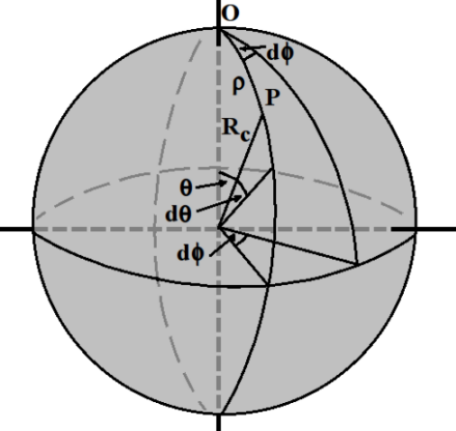
\includegraphics[width=0.5\textwidth]{./figures/2_theoretical_framework/2D_Sphere.png}
	
	\caption{\small{Métrica de una superficie esférica.}}
	
	\label{fig:HerschelModel}
\end{figure}
%.........................................................................



Un elemento de línea sobre la superficie puede ser descrito como


%.........................................................................
%Line element on the sphere
\eq{eq:LineElementSphere}
{ dl^2 = d\rho^2 + R_c^2 \sin^2 \pr{ \frac{\rho}{R_c}}d\phi^2 }
%.........................................................................


donde se ha introducido una nueva coordenada de longitud sobre la superficie
definida como $\rho = \theta R_c$ y $R_c$ radio de curvatura de la esfera. 
Otra forma muy conveniente de reescribir esta expresión y que permite una
generalización muy útil se logra introduciendo el parámetro de curvatura $k$ 
y la coordenada $r = \sin (\rho/a)$, obteniendo


%.........................................................................
%Line element on the sphere with time-dependent curvature
\eq{eq:Line}
{ dl^2 = a^2(t) \cor { \frac{dr^2}{1-kr^2} + r^2 d\phi^2 } }
%.........................................................................


por utilidad también se ha asumido un radio de curvatura dependiente del 
tiempo $R_c = a(t)$ y $k = -1$


	%---------------------------------------------------------------------
	%General relativity and Friedmann equations
	\subsection{Relatividad General y Ecuaciones de Friedmann}
	\label{subsec:GeneralRelativityAndFriedmannEquations}
	%---------------------------------------------------------------------
	

	%---------------------------------------------------------------------
	%Simple solutions of the universe
	\subsection{Simple Solutions of the Universe}
	\label{subsec:SimpleSolutionsOfTheUniverse}
	%---------------------------------------------------------------------


	%---------------------------------------------------------------------
	%Cosmological parameters
	\subsection{Cosmological Parameters}
	\label{subsec:CosmologicalParameters}
	%---------------------------------------------------------------------


%*************************************************************************




%*************************************************************************
%Nonlinear evolution and structure formation
\section{Nonlinear Evolution and Structure Formation}
\label{sec:NonlinearEvolutionAndStructureFormation}
%*************************************************************************




%*************************************************************************
%Quantification of cosmological environment
\section{Quantification of Cosmological Environment}
\label{sec:QuantificationOfCosmologicalEnvironment}


	%---------------------------------------------------------------------
	%The T-web method
	\subsection{The T-web Method}
	\label{subsec:TheT-webMethod}
	%---------------------------------------------------------------------


	%---------------------------------------------------------------------
	%The V-web method
	\subsection{The V-web Method}
	\label{subsec:TheV-webMethod}
	%---------------------------------------------------------------------


%*************************************************************************




%*************************************************************************
%The local group
\section{The Local Group}
\label{sec:TheLocalGroup}
%*************************************************************************